\documentclass[11pt,a4paper]{article}

% --- Essential Packages for pdfLaTeX ---
\usepackage[utf8]{inputenc}
\usepackage[T1]{fontenc}
\usepackage{lmodern}
\usepackage[margin=1in]{geometry}
\usepackage{graphicx}
\usepackage{booktabs}
\usepackage{amsmath,amssymb}
\usepackage{caption}
\usepackage{microtype}
\usepackage{hyperref}

\hypersetup{
    colorlinks=true,
    linkcolor=blue,
    urlcolor=blue,
    citecolor=blue
}

\begin{document}

% --- Header / Metadata ---
\noindent
\textbf{Author:} Trevor Robbins \hfill \textbf{Class:} CS 431/531 \\
\textbf{Project:} Calculating PI \hfill \textbf{Date:} \today

\vspace{1.5em}

% --- Title ---
\begin{center}
    {\LARGE \textbf{Analysis of OpenMP Parallelization for Calculating Digits of PI}}
\end{center}

\vspace{1em}

% --- Main Body (Original Text) ---
In this report, I conducted a case study for a serial vs parallel implementation of the Riemann Sum Algorithm (RSA) calculating the first $n$-digits of pi. On top of this, the codebase includes an implementation of the random variable Monte Carlo Method (MCM) for calculating pi, counting digits that fall inside a circle. Thread counts split across the parallel implementation depended on available CPU-cores, that being 2, 4, 8, 16, 32, and 64.

\vspace{0.75em}

For the Riemann Sum Algorithm, this involved integrating over a quarter circle for a sum of rectangular areas between the interval $[0, 1]$. This can be serially implemented, however partitioning the sums allows for a parallel implementation that splits rectangles across threads for the for loop itself.

\vspace{0.75em}

Moving onto the Monte Carlo Method, this simple technique is more of an analog for an incredibly educated guess. Using a randomly generated number between the interval of $[0, 1]$, our threads ``guess'' for an area inside of a unit circle that is contained within a square. Guesses outside the square are discarded, however the remaining ``right choices'' are added to our running ``hits'' variable sum. For this algorithm, I decided to try a hybrid bit-shifting with hashing approach to see if a speedup could be induced.

\vspace{1.5em}

% --- Results Section ---
\section*{Results}

In the results section, we will analyze the performance speedup from serial to parallel. As well as this, we will be using the scaling plot and benchmark data shown below:

\vspace{1em}

% Figure 1: Scaling PNG
\begin{figure}[htbp]
    \centering
    % Make sure 'scaling.png' is in the same folder as this .tex file
    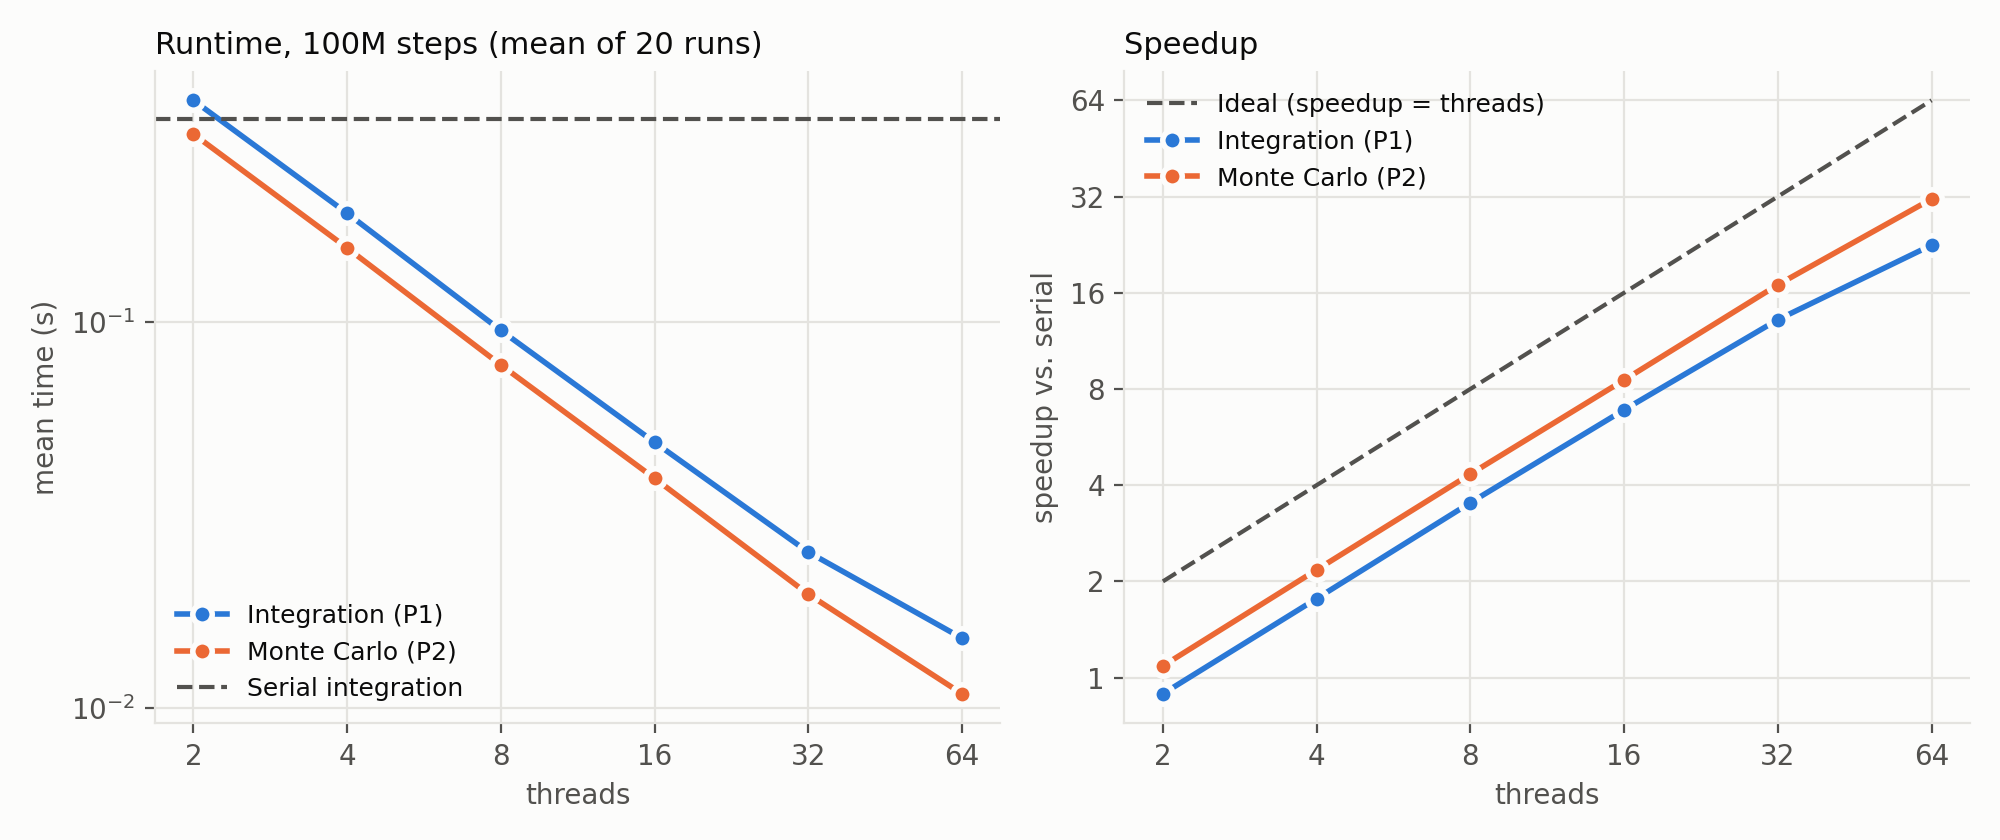
\includegraphics[width=0.92\textwidth]{scaling.png}
    \caption{Runtime (100M steps, mean of 20 runs) and speedup comparison vs. ideal linear scaling.}
    \label{fig:scaling}
\end{figure}

\vspace{1em}

% Figure 2 / Table: Benchmark Data from results.csv
\begin{table}[htbp]
    \centering
    \caption{Performance and speedup benchmarks across thread counts (100M steps, 20 runs).}
    \label{tab:results}
    \begin{tabular}{rcccccc}
        \toprule
        \textbf{Threads} & \textbf{Serial (s)} & \textbf{RSA P1 (s)} & \textbf{P1 Speedup} & \textbf{MCM P2 (s)} & \textbf{P2 Speedup} & \textbf{P1 Error} \\
        \midrule
        2  & 0.3352 & 0.3767 & 0.890$\times$  & 0.3081 & 1.088$\times$  & $1.021 \times 10^{-11}$ \\
        4  & 0.3393 & 0.1920 & 1.767$\times$  & 0.1561 & 2.174$\times$  & $1.021 \times 10^{-11}$ \\
        8  & 0.3363 & 0.0954 & 3.526$\times$  & 0.0776 & 4.333$\times$  & $1.021 \times 10^{-11}$ \\
        16 & 0.3365 & 0.0489 & 6.884$\times$  & 0.0394 & 8.536$\times$  & $1.021 \times 10^{-11}$ \\
        32 & 0.3345 & 0.0254 & 13.181$\times$ & 0.0197 & 16.952$\times$ & $1.021 \times 10^{-11}$ \\
        64 & 0.3423 & 0.0152 & 22.556$\times$ & 0.0109 & 31.441$\times$ & $1.021 \times 10^{-11}$ \\
        \bottomrule
    \end{tabular}
\end{table}

\vspace{1em}

Analyzing the results, the most surprising outcome was the massive speedup from the MCM to the RSA. Using the 64'th thread as the largest scaling example as thread counts increase, we can notice that its an almost 10x speedup over the RSA parallelization. I believe the reason behind this performance boost is due to two reasons. One is likely CPU-partitioning overhead, as analyzing the serial vs parallel RSA, the total time per thread scales better for the serial version, likely due to the lack of cost for context switching. Another reason could be the use of bit shifting for random-number generation rather than library calls, which could have sped up the result more than hypothesized. Regardless, taking a look at Figure~\ref{fig:scaling}, results scale linearly for input-size to thread ratio.

\end{document}